\documentclass{article}
\usepackage[utf8]{inputenc}
\usepackage[margin=2.6cm]{geometry}
\usepackage{float}
\usepackage{rotating}
\usepackage{graphicx}
\usepackage{caption}
\usepackage{subcaption}
\usepackage[round]{natbib}
\usepackage{setspace}
\usepackage{longtable}
\usepackage{lscape}
\onehalfspacing
\usepackage{tikz}
\usetikzlibrary{arrows,automata,positioning,shapes}
\usepackage{adjustbox}

\title{The interplay of resource acquisition and transfers explains the diversity of the female human life cycle.
\\
Registered Report}
\author{Pablo J. Varas Enriquez, Monique Borgerhoff Mulder, Heidi Colleran, Dieter Lukas*\\\\
* No special order of authors}
\date{\today}

\begin{document}

\maketitle

\tableofcontents

\section{Problem Formulation}

There are many paths an individual can follow through its life cycle, which is the basis of the diversity seen across the tree of life. The diversity of mortality schedules can lead to lifespans that vary from days to thousands of years (e.g. hairyback vs patagonian cypress \citep{balsamo1988life,lara19933620}) and reproductive outputs can go from a couple to thousands of offspring (e.g. eastern hemlock vs rain moth \citep{tindale1932revision,van2017lifetime}. Within the tree of life, the female human life cycle is characterized by a long lifespan and a short reproductive career, framed within long juvenile and post-reproductive stages \citep{kaplan2000theory}. Within these boundaries, the life cycle of female humans also varies in terms of mortality and fertility, with populations showing long lifespans and low reproductive output (e.g. post-demographic transition Japan \citep{de2017maximum}) or short lifespans and high reproductive output (e.g. foraging populations \citep{migliano2007life}). The diversity of life cycles observed among female human populations is fuelled by the differences in longevity and fertility between individuals within a population. However, it is not clear if the within-population variability of female human life cycles is also explained by the same processes that explain the differences among species across the tree of life. 
\\\\
The differences in life cycles between species have usually been related to the ways in which an individual allocates the limited resources available in its environment towards survival or reproduction \citep{stearns2000life}. In the case of humans, the differences in longevity at an individual level have been associated with resource availability (i.e. more resources equals longer lifespans) \citep{kaplan2003embodied}, while the relationship of fertility with resources is more complex \citep{mulder1998demographic,sear2016understanding}. Sharing dynamics have also been proposed as a key component to understand the different life cycles among female humans, due to the social nature of our species. Here, the presence of different members of the population have been associated with differences in the longevity and reproductive output of female individuals,as can be found in the literature related to cooperative breeding, sibling competition, female conflict, among others \citep{ivey2000cooperative,nitsch2013elder,mace2012female,sear2011much}. However, research in the area usually focus on specific components of the life cycle (e.g. longevity, number of offspring) rather than addressing them together, and/or black box the ways in which resources are available for female individuals (e.g. amount of food, presence of the grandmother). Therefore, the understanding of the mechanisms linking resources availability with the variability of life cycles within a female human population remains limited.
\\\\
Models that address these two limitations of how resource availability shape the life cycles of women in a population focus on the conditions that differentiate the female human life cycle from other species. The ``embodied capital model" suggests that the surplus of resource production during adulthood allows the evolution of the female human life cycle \citep{kaplan2000theory}. This model proposes that the difference between resource production and consumption allows high parental investment, translated in short interbirth intervals and long post-reproductive periods for the parents and long juvenile periods for their offspring. The ``pooled energy model" deepens in this framework by suggesting that alloparenting from individuals of different generations would allow to decrease the load of parental investment \citep{kramer2010pooled}. The ``inter-generational resource transfer model" poses that inter-generational transfers would play a major role in the mortality and fertility schedules of human populations. As developed by \cite{lee2003rethinking}, this model suggests that age-specific mortality is proportional to the remaining reproductive value and resource transfers made at later ages, predicting the early-life and later-life mortality patterns characteristics of the female human life cycle. Additionally, Chu and Lee further develop the ``Inter-generational resource transfer model", showing that transfers co-evolve with low mortality, since adults are more efficient to produce energy, which is transferred to juveniles, who are more efficient to turn that energy into body size, allowing lower mortality \citep{chu2006co}. While these models show that the female human life cycles co-evolved with the interplay of resource acquisition and transfers, they do not address how different resource dynamics can shape the variations of the life cycle within a population (see Fig.\ref{fig:1} for a graphical summary).
\\\\
Therefore, this project aims to develop a theoretical framework to understand how resource dynamics (i.e. resource production, consumption, transfer, storage) influence individual-level variations of the female human life cycle. The model would focus on a) how the life cycle of an individual varies under different resource dynamics across its lifespan, and b) how the variability of life cycles within a female human population changes due to differences in resource production, consumption, transfer, and storage. The framework will be developed with an agent-based model, because of its capacity to address complex phenomena from individual and population levels, as well as address stochasticity among individuals by allowing agents to behave differently despite being all under the same rules \citep{judson1994rise,wilensky2015introduction}. This last attribute of agent-based models is interesting for our purposes, because resource dynamics are understood as variables that play a role in the boundaries of variability of life cycles at an individual and population level. The model will be described using an ODD (Overview, Design concepts, Details) protocol, as an standardised way to clarify the scope, assumptions, and parameters used to answer our questions \citep{grimm2006standard,grimm2020odd}.

\section{Model description}

\subsection{Purpose and patterns}

The purpose of the model is to understand how different resource dynamics influence variations of the female life cycles within a population. The mechanism expected to influence the life cycle at an individual level is in the interplay of resource production, consumption, transfer, and storage which allows individuals to allocate resources for different life stage transition timings, reproductive timing and output within stages, and overall lifespan. Variability of the female human life cycle at the population level would be explained by the amount of different life cycles that arise from individual differences, which are based on the mechanism described earlier. The expected patterns can be described at an individual and at a population level. First, the life cycle of an individual should vary more due to differences in the amount of resources produced and consumed across the life cycle, while the sharing and storing dynamics would play a buffering role, by compensating the surplus and/or lack of resources that can be allocated in the life cycle from the other dynamics. Second, there should be less variability of life cycles in a population where individuals would have higher access to resources via receiving or production, higher storage capacity, and/or give less resources to other individuals. The variability of female life cycles in the population should be more sensitive to changes in resource production and consumption in comparison to sharing and storing resources (Table \ref{tab:1}).
\\\\
The life cycle of a female individual will be described by the time spent across five discrete stages (i.e. infant, juvenile, adult, reproductive-career, post-reproductive), which are defined by the timing of key events of the life course (i.e. age at weaning, age at menarche, age at first reproduction, age at menopause, and death). Longevity will also be a characteristic of the life cycle (i.e. number of years alive), as well as lifetime reproductive success (i.e. number of surviving offspring until sexual maturity). The influence of resource dynamics into the life cycle will be understood by the timing of reproductive events (i.e. age at first and last reproduction, and interbirth intervals) and life stage transitions (i.e. age at menarche, age at first reproduction, age at menopause). Finally, resource dynamics will be characterized by the amount of resources produced, transferred, consumed, and stored in each life cycle stage. A graphical representation can be seen in Fig. \ref{fig:2}.

\subsection{Entities, state variables, and scale}

\subsubsection{Entities}

Individuals represent females in a single-sex population. A single-sex population is used because the model is focused on the female human life cycle, under the assumption that it evolves independently from the male counterpart. Individuals that are born until they reach age of weaning are considered infants. Juveniles are individuals that transition from infants, until they reach age at menarche. Adults are individuals that have reached menarche until they have their first offspring or reach menopause. Adults transition to a reproductive-career stage once they have their first offspring, and remain in this stage until they reach menopause. From menopause onward individuals are considered post-reproductive.

\subsubsection{State variables}

Every individual in the simulation is characterised by state variables that are a) calculated new in each iteration, and b) modified from one iteration to the next:

\begin{itemize}
    \item Variables that are calculated new in each iteration:
    \begin{itemize}
        \item Resources produced: Amount of resources produced by the individual. The amount is fixed to each stage. Therefore, the individual whether produce resources (stage-specific resource production) or not ($0$) based on a stage-specific production probability specified during initialisation.
        \item Resources received: Amount of resources received by the individual from other individual(s). The amount received by another individual is fixed to each stage, and multiplied by the number of givers available in the population. The number of givers available depends on the amount of individuals that are giving resources in the iteration, constrained by specifications during initialisation.
        \item Resources consumed: Amount of resources consumed by the individual. The amount is fixed to each stage and specified during initialisation.
        \item Resources gave: Amount of resources given by the individual to other individual(s).The amount received by another individual is fixed to each stage, and multiplied by the number of givers available in the population. The number of givers available depends on the amount of individuals that are giving resources in the iteration, constrained by specifications during initialisation.
        \item Reproductive effort: Amount of resources the individual uses for reproduction, given the stage-specific probability. The amount is fixed to each stage. Therefore, the individual whether gives birth or not based on the stage-specific fertility probability and the amount of resources produced, received, consumed, gave, and stored.
    \end{itemize}
    \item Variables that are modified from one iteration to the next:
    \begin{itemize}
        \item Age: Amount of iterations the individual goes through from its birth until it dies. Age increases by one after each iteration, reflecting one year.
        \item Stage: Life cycle stage in which the individual is at the moment. There are five stages (infant, juvenile, adult, reproductive-career, post-reproductive), each with its own stage-specific resource and life-history dynamics. Individual progression through the stages is determined by the allocation of resources in the key event of transition.
        \item Resources stored: Amount of resources the individual stores for later in time (i.e. next iteration). The amount of resources stored depends on the surplus resources after the stage-specific resource and life-history dynamics. Therefore, the individual whether stores the surplus (stage-specific storing) or loses it (0) based on the stage-specific storing probability.
        \item Reproductive output: Amount of offspring produced, given the stage-specific fertility probability. Reproductive output increases by one after an iteration, if reproductive requirements (i.e. fertility probability and resources available) are met.
    \end{itemize}
\end{itemize}

\subsubsection{Auxiliary variables}

The individual dynamics are constrained by the following auxiliary variables. These variables are stage-specific, set at the initialisation and apply to all individuals in dependence on their state variables.

\begin{itemize}
    \item Die: Probability of dying in the life cycle stage. The probability distribution is based on the mortality rates from the cross-cultural study by \cite{gurven2007longevity}. The probability is adjusted according to the amount of resources stored by the individual. If there is a negative amount of resources stored, then the individual automatically dies.
    \item Produce: Probability of producing resources. The probability is based on a binomial distribution regarding whether the individual produces resources ($1$) or not ($0$). The values of the distribution are based on \cite{koster2020life}.
    \item Receive: Probability of receiving resources from another individual(s). The probability is based on a distribution starting in zero and a maximum value based on \cite{gurven2004give}.
    \item Consume: Amount of resources necessary for somatic maintenance, based on \cite{kaplan2000theory,pontzer2021daily}.
    \item Store: Probability of storing the surplus of resources from production and sharing dynamics at the end of an iteration. The probability is based on a binomial distribution regarding whether the individual stores resources ($1$) or not ($0$). The values of the distribution are based on \citep{bowles2011cultivation}.
    \item Give: Probability of giving resources to another individual(s). The probability is based on a distribution starting in zero and a maximum value based on \cite{gurven2004give}.
    \item Reproduce: Probability of producing a offspring. The probability is based on a stage-specific fertility rate, which is adjusted according to the resources available for an individual.
    \item Transition: Probability of transitioning to the next stage. The transitions are specified as follow:
    \begin{itemize}
        \item Infant transition: Reaching the growth and development necessary for weaning and transition to the juvenile stage. The probability distribution is based on the values in \cite{wood2017dynamics}.
        \item Sexual maturity: Reaching the development necessary for menarche and transition to the adult stage. The probability distribution is based on the values in \cite{mulder1989menarche} and \cite{kramer2010teen}.
        \item Reproduce (adult stage): Producing your first offspring and transition to the reproductive-career stage. The values of the distribution are based on the work of \cite{wood2017dynamics}.
        \item Menopause: Reaching the moment where you cannot, biologically, produce more offspring and transition to the post-reproductive stage. The values of age at menopause are based on \cite{laisk2019demographic}.
    \end{itemize}
\end{itemize}

\subsubsection{Scale}

Each iteration in the model represents one year. The probabilities  of producing and storing are binomial, with the values of happening ($1$) or not ($0$). The probabilities of receiving and giving are discrete, with a minimum of zero (i.e. no receiving/giving) and a maximum based on cross-cultural values. The amount of resources an individual produces, receives, consumes, gives, and store are stage-specific. Reproductive effort is evaluated after the resource dynamics, followed by the evaluation for stage transition. Finally, the amount or resources available are stored and passed from one year to the next, being evaluated for survival at the beginning of the iteration.

\subsection{Process overview and scheduling}

Every sub model described in the following process is stage-specific. Infant individuals go through survival, receiving, consuming, and storing sub models each year until they transition to the next stage. Once in the juvenile stage, individuals go through survive, produce, receive, consume, give, and store sub models for each year until they reach sexual maturity, transitioning to the adult stage. In the adult stage, individuals go through surviving, producing, receiving, consuming, giving, and storing sub models until they have their first offspring or reach menopause. If an adult transition to a reproductive-career stage, it goes through surviving, producing, receiving, consuming, giving, storing sub models and also through a reproduction sub model until it reaches menopause. Once in a post-reproductive stage, the individual goes through the surviving, producing, receiving, consuming, giving, and storing sub models of the stage. In each year, the individual increase its age and updates the amount of resources it has. During each transition, the individual updates its stage variable and also transitions with the resources it has stored from the earlier stage.
\\\\
The scheduling of the process starts with the survival sub model so only individuals who survive can age and go through the rest of the sub models in the iteration. The resource-related sub models start with those who may increase the amount of resources available (production and receiving), followed by those who decrease the amount of resources (consumption and giving), and ending with the storing sub model. The reproduction sub model follows the resource-related ones in order to see the influence of resource dynamics in the reproductive output and timing. The schedule ends with the transition sub model to evaluate if the individual moves to the next life cycle stage or not.

\subsection{Design concepts}

\subsubsection{Basic principles}

The model aims to understand how the variability of life cycles within a population change based on the influence of different resource dynamics. Models so far have focused on the conditions under which the female human life cycle evolved (e.g. embodied capital model \citep{kaplan1996theory} or resource transfer model \citep{chu2006co}), while the model differs from them by focusing in the mechanisms behind the variability of life cycles. Additionally, the model is more explicit in the resource dynamics than previous models \citep{price2020fitness,kaplan1996theory,chu2006co,lee2003rethinking,kramer2010pooled}. First, resource transfers are defined more general, and not bounded to specific relationships among individuals (e.g. parent-offspring transfers as in \cite{kaplan1996theory} or downward adult-juvenile transfers as in \cite{chu2006co}). Second, resource transfers are modelled independently instead as a byproduct of other resource dynamics (e.g. giving as a positive outcome from resource production and consumption, and receiving as a negative one, as in \cite{lee2003rethinking,chu2006co}). Finally, the model is driven by mechanistic processes since the individual survives, reproduce, and transition through the life cycle depending on the amount of resources it has, but it is also stochastic since agents take random decisions on whether allocate resource into the life cycle or not (see Stochasticity section below for further details). Therefore, the variability observed as outcome of the model rises from individual stochastic decisions instead of fitness maximization.

\subsubsection{Emergence}

The life cycle of an individual emerges from its behaviour. The life cycle is represented by the timing of key events of the life course (i.e. life stage transition, reproductive output and timing, and longevity) constrained by the stage-specific sub models related to resource dynamics. Population dynamics emerge from the behaviour of the individuals. The population dynamics are represented as the age distributions of the life cycle transitions, reproductive output and timing, and longevity and surviving individuals. The aim is to understand how the resource dynamics (i.e. production, consumption, transfer, storage) experienced by individuals within a population cause changes in the variability of different components of the female human life cycle (i.e. survival, age at menarche, age at first reproduction, number of offspring, interbirth intervals, age at last reproduction, age at menopause, longevity).

\subsubsection{Adaptation}

The model has three adaptive behaviours, that characterise the female human life cycle: 1) the time to transition from one life stage to another, 2) the reproductive output and timing, and 3) longevity. The three of them are based on a random decision of the individual to whether or not transition, reproduce, and/or survive as well as the amount of resource the individual has from the resource dynamics it experiences in each iteration.

\subsubsection{Objectives}

Not apply

\subsubsection{Learning}

There is no learning process for the individuals in the population because the model focuses on the biological constraints under which the female human life cycle varies.

\subsubsection{Prediction}

The adaptive behaviour of an individual is based on the implicit prediction that moving to the next life stage, reproducing, and/or surviving when having the necessary amount of resources as well as a successful outcome from the random decision process is likely to eventually result in individuals having a life cycle that has the longest lifespan, and the highest reproductive output. This life cycle would be possible by expanding their time in the reproductive career stage (i.e. reaching sexual maturity and starting reproduction earlier, while stopping reproduction and reaching menopause later). On the other extreme, individuals are likely to have life cycle with short lifespan and low reproductive output when they do not have enough resources and have unsuccessful outcomes from the random decision process. This life cycle would have long time before reaching sexual maturity and starting reproduction, while it would stop reproduction and reach menopause earlier. Variations of these predictions can be expected by differences in the amount of resources and successful outcomes from the random processes that an individual experiences through its life cycle, being more sensitive to changes in resource production and consumption, whereas sharing and storing dynamics should have a buffering effect.
\\\\
At the population level, it should be expected that variability of life cycles is lower in populations where individuals are more homogeneous in the resource dynamics they experience (i.e. the two extremes described above), while the variability increases as individuals are more likely to experience different amounts of resources and outcomes from their decision processes, especially by differences in resource production and consumption.

\subsubsection{Sensing}

Individuals are assumed to know their stage, and their current resources produced, consumed, received, gave, and stored in order to allocate them into reproduction, survival, and/or transitioning from one life cycle stage to another.

\subsubsection{Interaction}

Not apply

\subsubsection{Stochasticity}

Resource dynamics and the allocation of them towards different key components of the female human life cycle are stochastic in the model since they are based on probability distributions. Individuals produce, receive, consume, give, and store resources within an iteration based on having a successful outcome ($1$) from a binomial distribution, which is totally random. Individuals survive, reproduce, and transition from one life stage to another not automatically by reaching a certain amount of resources, they also need to have a successful outcome ($1$) from a binomial distribution to allocate those resources, which also is totally random. Therefore, decisions are stochastic within the constrains of resources available for the individual.

\subsubsection{Collectives}

Not apply

\subsubsection{Observation}

The purpose of the model is to identify which scenarios of resource acquisition and transfers vary the timing of life stage transitions, longevity, and reproductive timing and output of individuals. Therefore, the different resource dynamics (i.e. production, consumption, giving, receiving, storing) and the timing and output of the different components of the life cycle are recorded for each individual. At the population level, distributions of each trait of the female human life cycle as well as resource dynamics are produced based on the individual data.

\subsection{Initialization}

At initialisation, the population will be composed of equal number of individuals per life cycle stage. Each infant individual in the initial population have the baseline resources to survive to guarantee the survival in the first survival sub model and go through the resource dynamics sub models, only ageing after surviving the survival sub model in the next iteration.
\\\\
The auxiliary variables for each stage are set at initialisation. The values for each variable and stage are based on previous research (Table \ref{tab:1}).

\subsection{Input Data}

The model does not use input data to represent time-varying processes.

\subsection{Sub models}

Each individual alive in a given iteration goes through all the sub models specific to the life stage that it is in.

\begin{itemize}
    \item Infant
    \begin{itemize}
        \item Die: The infant survives by sampling a value equal or lower than the stage-specific survival rate, based on \cite{gurven2007longevity}. If the individual samples a value lower than the stage-specific survival rate, then it dies. The infant has a higher chance to survive if it has a larger amount of resources stored from the previous iteration. The individual automatically dies in case the amount of resources stored is negative. The amount of resources stored decreases by the costs of survival.
        \item Receive: The individual receives the amount of resources multiplied by the number of givers available to it. The amount of resources per giver is fixed, stage-specific, and based on \cite{gurven2004give}. The number of givers is based on sampling a value between zero and the maximum number of givers in \cite{gurven2004give}, constrained by the number of individuals in the population that have a successful outcome from the \emph{Give} sub model. If the value sampled is zero, then the individual does not receive resources in that iteration.
        \item Consume: The infant consumes the amount of resources necessary for somatic maintenance from the resources the individual acquires from the sub models \emph{Receive} and \emph{Store} in the iteration, based on \cite{kaplan2000theory, pontzer2021daily}.
        \item Store: The infant has a probability of storing the surplus of resources available in the iteration by sampling from a binomial distribution. The individual either stores ($1$) or not ($0$), based on the values in \citep{bowles2011cultivation}. In case the individual does not store ($0$) then the surplus  of resources in the iteration is lost.
        \item Transition: The infant transition by sampling a value equal or lower than the stage-specific probability of weaning, based on the values on \cite{wood2017dynamics}. The infant has a higher chance to transition if it has a larger amount of resources from the \emph{Receive} and \emph{Store} sub models. The amount of resources decreases by the costs of transition, while the remaining amount is stored, and transition to the juvenile stage.
    \end{itemize}
    \item Juvenile
    \begin{itemize}
        \item Die: The juvenile survives by sampling a value equal or lower than the stage-specific survival rate, based on \cite{gurven2007longevity}. If the individual samples a value lower than the stage-specific survival rate, then it dies. The juvenile has a higher chance to survive if it has a larger amount of resources stored from the previous iteration. The individual automatically dies in case the amount of resources stored is negative. The amount of resources decreases by the costs of survival.
        \item Produce: The juvenile has a probability of producing by sampling from a binomial distribution. The individual either produces resources ($1$) or not ($0$), and the amount of resources produced is fixed, stage-specific, and based on \cite{koster2020life}.
        \item Receive: The individual receives the amount of resources multiplied by the number of givers available to it. The amount of resources per giver is fixed, stage-specific, and based on \cite{gurven2004give}. The number of givers is based on sampling a value between zero and the maximum number of givers in \cite{gurven2004give}, constrained by the number of individuals in the population that have a successful outcome from the \emph{Give} sub model. If the value sampled is zero, then the individual does not receive resources in that iteration.
        \item Consume: The juvenile consumes the amount of resources necessary for somatic maintenance from the resources the individual acquires from the sub models \emph{Produce}, \emph{Receive} and \emph{Store} in the iteration, based on \cite{kaplan2000theory, pontzer2021daily}.
        \item Give: The individual gives the amount of resources multiplied by the number of receivers available to it. The amount of resources per receiver is fixed, stage-specific, based on \cite{gurven2004give}. The number of receivers is based on sampling a value between zero and the maximum number of receivers in \cite{gurven2004give}, constrained by the number of individuals in the population that have a successful outcome from the \emph{Receive} sub model. If the value sampled is zero, then the individual does not give resources in that iteration.
        \item Store: The juvenile has a probability of storing the surplus of resources available in the iteration by sampling from a binomial distribution. The individual either stores ($1$) or not ($0$), based on the values on \citep{bowles2011cultivation}. In case the individual does not store ($0$) then the surplus of resources in the iteration is lost.
        \item Age at sexual maturity: The juvenile transition by sampling a value equal or lower than the stage-specific probability of reaching sexual maturity, based on the values on \citep{ellison2017reproductive}. The juvenile has a higher chance to be sexually mature if it has a larger amount of resources available from the resource-related sub models of the iteration. The amount of resources decreases by the costs of transition, while the remaining amount is stored, and transition to the adult stage.
    \end{itemize}
    \item Adult
    \begin{itemize}
        \item Die: The adult survives by sampling a value equal or lower than the stage-specific survival rate, based on \cite{gurven2007longevity}. If the individual samples a value lower than the stage-specific survival rate, then it dies. The adult has a higher chance to survive if it has a larger amount of resources stored from the previous iteration. The individual automatically dies in case the amount of resources stored is negative. The amount of resources decreases by the costs of survival.
        \item Produce: The adult has a probability of producing by sampling from a binomial distribution. The individual either produces resources ($1$) or not ($0$), and the amount of resources produced is fixed, stage-specific, and based on \cite{koster2020life}.
        \item Receive: The individual receives the amount of resources multiplied by the number of givers available to it. The amount of resources per giver is fixed, stage-specific, and based on \cite{gurven2004give}. The number of givers is based on sampling a value between zero and the maximum number of givers in \cite{gurven2004give}, constrained by the number of individuals in the population that have a successful outcome from the \emph{Give} sub model. If the value sampled is zero, then the individual does not receive resources in that iteration.
        \item Consume: The adult consumes the amount of resources necessary for somatic maintenance from the resources the individual acquires from the sub models \emph{Produce}, \emph{Receive} and \emph{Store} in the iteration, based on \cite{kaplan2000theory, pontzer2021daily}.
        \item Give: The individual gives the amount of resources multiplied by the number of receivers available to it. The amount of resources per receiver is fixed, stage-specific, based on \cite{gurven2004give}. The number of receivers is based on sampling a value between zero and the maximum number of receivers in \cite{gurven2004give}, constrained by the number of individuals in the population that have a successful outcome from the \emph{Receive} sub model. If the value sampled is zero, then the individual does not give resources in that iteration.
        \item Store: The adult has a probability of storing the surplus of resources available in the iteration by sampling from a binomial distribution. The individual either stores ($1$) or not ($0$), based on the values on \citep{bowles2011cultivation}. In case the individual does not store ($0$) then the surplus is lost.
        \item Transition: The adult transition either to a reproductive stage (i.e. reproductive career) or a post-reproductive stage depending if the individual either have an offspring or reaches menopause, respectively.
        \begin{itemize}
            \item Age at first reproduction: The adult reproduce by sampling from a Poisson distribution a value equal or lower than the stage-specific fertility rate, based on the values on \citep{wood2017dynamics}. If the individual samples a value equal or lower than the stage-specific fertility rate, then it produces one offspring. The individual in its reproductive career has a higher chance to have an offspring if it has a larger amount of resources from the \emph{Produce}, \emph{Receive}, \emph{Consume}, \emph{Give}, and \emph{Store} sub models. The amount of resources decreases by the costs of reproduction \citep{wood2017dynamics}, while the remaining amount is stored, and transition to the breeding stage.
            \item Menopause: The adult transitions by sampling a value equal or lower than the stage-specific probability of menopause, based on the values on \citep{laisk2019demographic}. The individual in its reproductive career has a lower chance to transition if it has a larger amount of resources from the \emph{Produce}, \emph{Receive}, \emph{Consume}, \emph{Give}, and \emph{Store} sub models, where the chance increases every iteration. The amount of resources decreases by the costs of menopause, while the remaining amount is stored, and transition to the post-reproductive stage.
        \end{itemize}
    \end{itemize}
    \item Reproductive career
    \begin{itemize}
        \item Die: The individual in its reproductive career survives by sampling a value equal or lower than the stage-specific survival rate, based on \cite{gurven2007longevity}. If the individual samples a value lower than the stage-specific survival rate, then it dies. The individual has a higher chance to survive if it has a larger amount of resources stored from the previous iteration. The individual automatically dies in case the amount of resources stored is negative. The amount of resources decreases by the costs of survival.
        \item Produce: The individual in its reproductive career has a probability of producing by sampling from a binomial distribution. The individual either produces resources ($1$) or not ($0$) and the amount of resources produced is fixed, stage-specific, and based on \cite{koster2020life}.
        \item Receive: The individual receives the amount of resources multiplied by the number of givers available to it. The amount of resources per giver is fixed, stage-specific, and based on \cite{gurven2004give}. The number of givers is based on sampling a value between zero and the maximum number of givers in \cite{gurven2004give}, constrained by the number of individuals in the population that have a successful outcome from the \emph{Give} sub model. If the value sampled is zero, then the individual does not receive resources in that iteration. 
        \item Consume: The individual consumes the amount of resources necessary for somatic maintenance from the resources the individual acquires from the sub models \emph{Produce}, \emph{Receive} and \emph{Store} in the iteration, based on \cite{kaplan2000theory, pontzer2021daily}.
        \item Give: The individual gives the amount of resources multiplied by the number of receivers available to it. The amount of resources per receiver is fixed, stage-specific, based on \cite{gurven2004give}. The number of receivers is based on sampling a value between zero and the maximum number of receivers in \cite{gurven2004give}, constrained by the number of individuals in the population that have a successful outcome from the \emph{Receive} sub model. If the value sampled is zero, then the individual does not give resources in that iteration.
        \item Store: The individual in its reproductive career has a probability of storing the surplus of resources available in the iteration by sampling from a binomial distribution. The individual either stores ($1$) or not ($0$), based on the values on \citep{bowles2011cultivation}. In case the individual does not store ($0$) then the surplus is lost.
        \item Reproduce: The individual in its reproductive career produce an offspring by sampling from a Poisson distribution a value equal or lower than the stage-specific fertility rate, based on the values on \citep{wood2017dynamics}. If the individual samples a value equal or higher than the stage-specific fertility rate, then it produces one offspring. The individual in its reproductive career has a higher chance to have an offspring if it has a larger amount of resources from the \emph{Produce}, \emph{Receive}, \emph{Consume}, \emph{Give}, and \emph{Store} sub models. The amount of resources decreases by the costs of reproduction \citep{wood2017dynamics}, which increases after every reproduction.
        \item Menopause: The individual in its reproductive career transition by sampling a value equal or lower than the stage-specific probability of menopause, based on the values on \citep{laisk2019demographic}. The individual in its reproductive career has a lower chance to transition if it has a larger amount of resources from the \emph{Produce}, \emph{Receive}, \emph{Consume}, \emph{Give}, and \emph{Store} sub models, where the chance increases every iteration. The amount of resources decreases by the costs of menopause, while the remaining amount is stored, and transition to the post-reproductive stage.
    \end{itemize}
    \item Post-reproductive
    \begin{itemize}
        \item Die: The post-reproductive survives by sampling a value equal or lower than the stage-specific survival rate, based on \cite{gurven2007longevity}. If the individual samples a value lower than the stage-specific survival rate, then it dies. The post-reproductive has a higher chance to survive if it has a larger amount of resources stored from the previous iteration. The individual automatically dies in case the amount of resources stored is negative. The amount of resources decreases by the costs of survival.
        \item Produce: The post-reproductive has a probability of producing by sampling from a binomial distribution. The individual either produces resources ($1$) or not ($0$), and the amount of resources produced is fixed, stage-specific, and based on \cite{koster2020life}.
        \item Receive: The individual receives the amount of resources multiplied by the number of givers available to it. The amount of resources per giver is fixed, stage-specific, and based on \cite{gurven2004give}. The number of givers is based on sampling a value between zero and the maximum number of givers in \cite{gurven2004give}, constrained by the number of individuals in the population that have a successful outcome from the \emph{Give} sub model. If the value sampled is zero, then the individual does not receive resources in that iteration.
        \item Consume: The post-reproductive consumes the amount of resources necessary for somatic maintenance from the resources the individual acquires from the sub models \emph{Produce}, \emph{Receive} and \emph{Store} in the iteration, based on \cite{kaplan2000theory, pontzer2021daily}.
        \item Give: The individual gives the amount of resources multiplied by the number of receivers available to it. The amount of resources per receiver is fixed, stage-specific, based on \cite{gurven2004give}. The number of receivers is based on sampling a value between zero and the maximum number of receivers in \cite{gurven2004give}, constrained by the number of individuals in the population that have a successful outcome from the \emph{Receive} sub model. If the value sampled is zero, then the individual does not give resources in that iteration.
        \item Store: The post-reproductive has a probability of storing the surplus of resources available in the iteration by sampling from a binomial distribution. The individual either stores ($1$) or not ($0$), based on the values on \citep{bowles2011cultivation}. In case the individual does not store ($0$) then the surplus is lost.
    \end{itemize}
\end{itemize}

\section{Model Analysis}

The model analysis consists on running simulations where the resource dynamics are considered the input parameters while the components of the life cycle are the output. Different combinations of resource dynamics will be used to analyse the influence of each input parameters in the variability of female life cycles, recording them at the individual and population level. Three levels for each resource dynamic (high, medium, low) are considered to define the different scenarios of resource dynamics. Regarding the components of the life cycle, the timing of life stage transitions, reproductive output and timing, and longevity will be recorded for each individual. Additionally, distributions will be built from the individual records to estimate the variability of the different components of the life cycle. Finally, multi-variate multi-level models will be built to analyze how the different resource dynamics shape variations in the female human life cycle at the individual and population level.

\section{Future modifications}

The model might be modified in order to include inter-generational resource transfers, which would allow to consider the life cycle stage with whom the individual gives and/or receives resources. This is not only based in the theoretical models developed so far \citep{lee2003rethinking,chu2006co} but also in empirical studies that suggest that the direction and with whom the resource transfer is done might be crucial to understand the role of sharing dynamics in the female human life cycle \citep{hooper2015inclusive,jones2015resource}.

\section{Tables and Figures}

\begin{figure}[H]
\centering
\begin{minipage}{.47\textwidth}
\centering
\vfill
  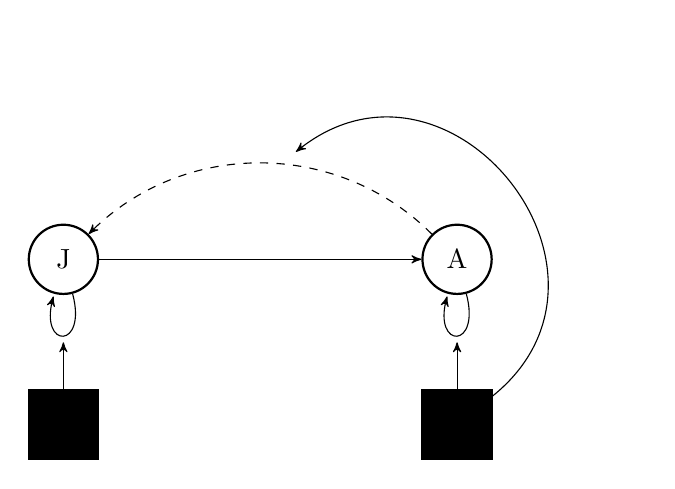
\begin{tikzpicture}[->,>=stealth',auto,thin]
\tikzstyle{every state}=[fill=white,shape=rectangle,draw,thick,text=black, text centered, text width=0.5cm, align=center]

\node[state]        (A) [shape=circle]        {J};
\node[state]		(B) [below of=A,node distance=0.6cm,draw=none,fill=none] {};
\node[state]		(C) [below of=B,node distance=1.5cm,fill=black] {};
\node[state]        (D) [right of=A,shape=circle, node distance=5cm] {A};
\node[state]		(E) [below of=D,node distance=0.6cm,draw=none,fill=none] {};
\node[state]		(F) [below of=E,node distance=1.5cm,fill=black] {};
\node[state]        (G) [right of=A,node distance=2.5cm,draw=none,fill=none] {};
\node[state]        (H) [above of=G,node distance=1cm,draw=none,fill=none] {};

\path
(A) edge[loop below] (A)
(C) edge (B)
(A) edge (D)
(D) edge[loop below] (D)
(D) edge[dashed,bend left=-45] (A)
(F) edge (E)
(F) edge[bend right=90, min distance=2.5cm] (H)
;
    \end{tikzpicture}
 \vfill
\captionsetup{labelformat=empty}
\caption{1) Black box resource dynamics model}
\label{fig:blackbox}
\vspace{\baselineskip}
\end{minipage}\qquad
\begin{minipage}{.47\textwidth}
\centering
\vfill
\begin{tikzpicture}[->,>=stealth',auto,thin,]
\tikzstyle{every state}=[fill=white,shape=rectangle,draw,thick,text=black, text centered, text width=0.5cm, align=center]

\node[state]        (A) [shape=circle]        {J};
\node[state]		(B) [below of=A,node distance=0.6cm,draw=none,fill=none] {};
\node[state]		(C) [below left of=B,node distance=1.5cm] {R$_J$};
\node[state]        (D) [below right of=B,node distance=1.5cm] {S$_J$};
\node[state]        (E) [right of=A, node distance=5cm,shape=circle] {A};
\node[state]		(F) [below of=E,node distance=0.6cm,draw=none,fill=none] {};
\node[state]		(G) [below left of=F,node distance=1.5cm] {G$_A$};
\node[state]		(I) [below of=F,node distance=2.5cm] {P$_A$};
\node[state]        (J) [below right of=F,node distance=1.5cm] {S$_A$};
\node[state]        (K) [right of=A,node distance=2.5cm,draw=none,fill=none] {};
\node[state]        (L) [above of=K,node distance=1cm,draw=none,fill=none] {};

\path
(A) edge[loop below] (A)
(C) edge (D)
(D) edge (B)
(C) edge (D)
(A) edge (E)
(E) edge[loop below] (E)
(E) edge[dashed,bend left=-45] (A)
(I) edge (G)
(I) edge (J)
(I) edge[bend right=100, min distance=4cm] (L)
(J) edge (F)
;
    \end{tikzpicture}
\vfill
\captionsetup{labelformat=empty}
\caption{2) Embodied capital model}
\label{fig:embodied}
\end{minipage}

\begin{minipage}{.41\textwidth}
\centering
\vfill
      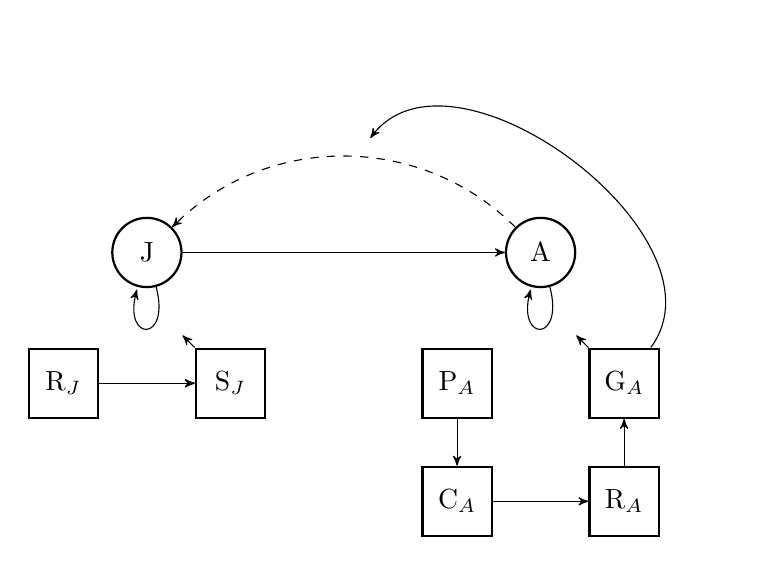
\begin{tikzpicture}[->,>=stealth',auto,thin]
\tikzstyle{every state}=[fill=white,shape=rectangle,draw,thick,text=black, text centered, text width=0.5cm, align=center]

\node[state]        (A) [shape=circle]        {J};
\node[state]		(B) [below of=A,node distance=0.6cm,draw=none,fill=none] {};
\node[state]		(C) [below left of=B,node distance=1.5cm] {R$_J$};
\node[state]        (D) [below right of=B,node distance=1.5cm] {S$_J$};
\node[state]        (E) [right of=A, node distance=5cm,shape=circle] {A};
\node[state]		(F) [below of=E,node distance=0.6cm,draw=none,fill=none] {};
\node[state]		(G) [below left of=F,node distance=1.5cm] {P$_A$};
\node[state]		(I) [below of=G,node distance=1.5cm] {C$_A$};
\node[state]        (J) [below right of=F,node distance=1.5cm] {G$_A$};
\node[state]        (K) [below of=J,node distance=1.5cm,] {R$_A$};
\node[state]        (L) [right of=A,node distance=2.5cm,draw=none,fill=none] {};
\node[state]        (M) [above of=L,node distance=1cm,draw=none,fill=none] {};

\path
(A) edge[loop below] (A)
(C) edge (D)
(D) edge (B)
(C) edge (D)
(A) edge (E)
(E) edge[loop below] (E)
(E) edge[dashed,bend left=-45] (A)
(G) edge (I)
(I) edge (K)
(J) edge[bend right=90, min distance=1.5cm] (M)
(J) edge (F)
(K) edge (J)
;
    \end{tikzpicture}
 \vfill
\captionsetup{labelformat=empty}
\caption{3) Inter-generational resource transfer model}
\label{fig:transfer}
\end{minipage}\qquad
\begin{minipage}{.5\textwidth}
\centering
\vfill
    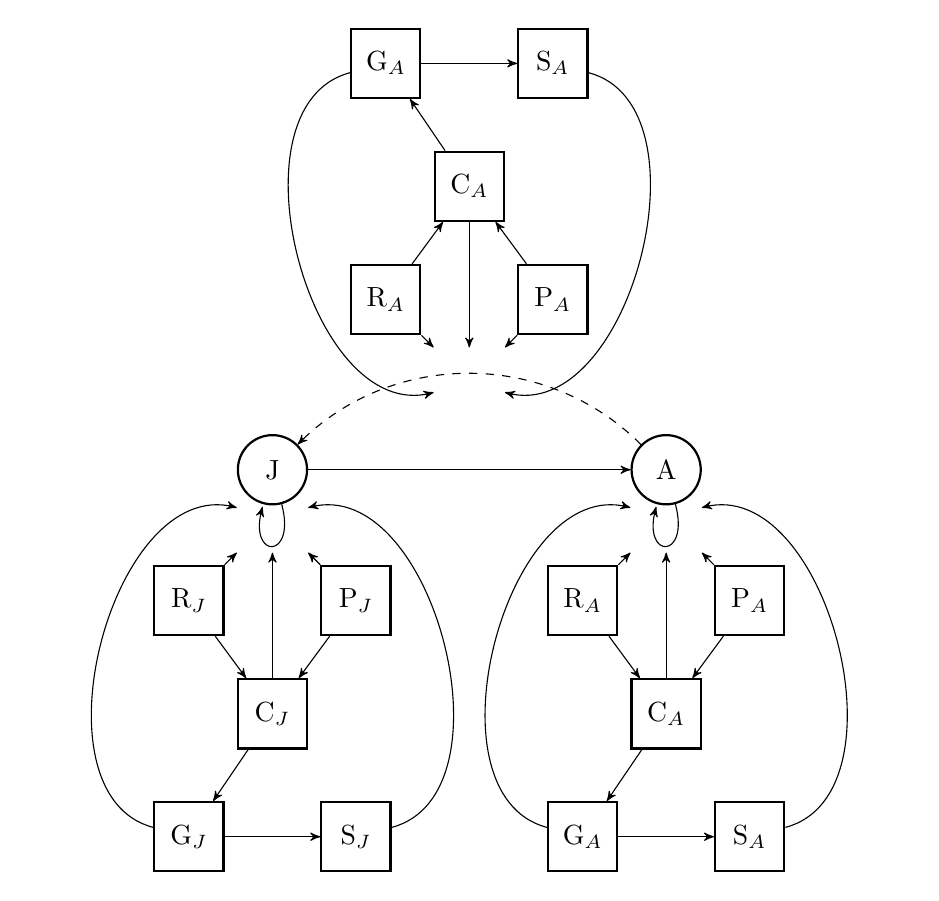
\begin{tikzpicture}[->,>=stealth',auto,thin]
\tikzstyle{every state}=[fill=white,shape=rectangle,draw,thick,text=black, text centered, text width=0.5cm, align=center]

\node[state]        (A) [shape=circle]        {J};
\node[state]		(B) [below of=A,node distance=0.6cm,draw=none,fill=none] {};
\node[state]		(C) [below left of=B,node distance=1.5cm] {R$_J$};
\node[state]        (D) [below of=C,node distance=3cm] {G$_J$};
\node[state]		(E) [below of=B,node distance=2.5cm] {C$_J$};
\node[state]        (F) [below right of=B,node distance=1.5cm] {P$_J$};
\node[state]		(G) [below of=F,node distance=3cm] {S$_J$};
\node[state]        (H) [right of=A, node distance=5cm,shape=circle] {A};
\node[state]		(I) [below of=H,node distance=0.6cm,draw=none,fill=none] {};
\node[state]		(J) [below left of=I,node distance=1.5cm] {R$_A$};
\node[state]		(K) [below of=J,node distance=3cm] {G$_A$};
\node[state]		(L) [below of=I,node distance=2.5cm] {C$_A$};
\node[state]        (M) [below right of=I,node distance=1.5cm] {P$_A$};
\node[state]		(N) [below of=M,node distance=3cm] {S$_A$};
\node[state]        (O) [right of=A,node distance=2.5cm,draw=none,fill=none] {};
\node[state]        (P) [above of=O,node distance=1.1cm,draw=none,fill=none] {};
\node[state]		(Q) [above left of=P,node distance=1.5cm] {R$_A$};
\node[state]		(R) [above of=Q,node distance=3cm] {G$_A$};
\node[state]		(S) [above of=P,node distance=2.5cm] {C$_A$};
\node[state]        (T) [above right of=P,node distance=1.5cm] {P$_A$};
\node[state]		(U) [above of=T,node distance=3cm] {S$_A$};

\path
(A) edge[loop below] (A)
(C) edge (B)
(C) edge (E)
(D) edge[bend right=-90] (B)
(D) edge (G)
(E) edge (B)
(E) edge (D)
(F) edge (B)
(F) edge (E)
(G) edge[bend left=-90] (B)
(A) edge (H)
(H) edge[loop below] (H)
(H) edge[dashed,bend left=-45] (A)
(J) edge (I)
(J) edge (L)
(K) edge[bend right=-90] (I)
(K) edge (N)
(L) edge (I)
(L) edge (K)
(M) edge (I)
(M) edge (L)
(N) edge[bend left=-90] (I)
(Q) edge (P)
(Q) edge (S)
(R) edge[bend left=-90] (P)
(R) edge (U)
(S) edge (P)
(S) edge (R)
(T) edge (P)
(T) edge (S)
(U) edge[bend right=-90] (P)
;
    \end{tikzpicture}
\vfill
\captionsetup{labelformat=empty}
\caption{4) Proposed model}
\label{fig:ourmodel}
\end{minipage}
\setcounter{figure}{0}
    \caption{Graphical representation of the different approaches used to understand the relationship between resources and the female human life cycle. \ref{fig:blackbox}) is the black boxing of resource dynamics. \ref{fig:embodied}) is the embodied capital approach, where individuals produce resources that are invested in embodied capital or their offspring. \ref{fig:transfer}) is the inter-generational resource transfer model, where the output of production and consumption is transferred from adults to juveniles. \ref{fig:ourmodel}) is the proposed model, where each resource dynamic has an independent influence on the life cycle. J and A represent juvenile and adult life stages, respectively. Loop arrows below life cycle stages refers to survival and the dashed arrows to reproduction. The resource dynamics are production (P), consumption (C), receiving (R), giving (G), and storing (S). The thick arrows represent the relationship between two elements.}
    \label{fig:1}
    
\end{figure}

\begin{table}[H]
    \centering
    \caption{Summary of the study design. \emph{Question} is where are the research questions driving the development of the model. \emph{Hypothesis} is where are the predictions answering the research questions. \emph{Analysis plan} is where the tests used to answer the research question are described. \emph{Interpretation} is a description of possible different outcomes, and their interpretation in relation to the hypothesis. \emph{Contested theory} is a description on how the possible outcomes could prove wrong or show incomplete current theories.}
    \begin{adjustbox}{width=\textwidth}
    \begin{tabular}{p{4cm}p{4cm}p{4cm}p{4cm}p{4cm} }
    \hline
    Question & Hypothesis & Analysis plan & Interpretation & Contested Theory \\ 
    \hline
    How does the life cycle of an individual varies by different resource dynamics? & An individual life cycle should vary more by the dynamics of resource production and consumption, while sharing and storing dynamics have a buffering effect & Multi-variate and multi-level models based on the different resource dynamic combinations and key components of the life cycle of an individual & An individual that experiences higher amount of resources and more successful random decisions is likely to live longer and reproduce more by expanding their time in the reproductive career stage. An individual that experiences less resources and successful random decisions is likely to life shorter and reproduce less by shrinking their reproductive career stage. Sharing and storing dynamics should decrease the impact in both cases. & The results would synthesis the theories developed from the embodied and inter-generational transfer models, by accounting for embodied capital (i.e. storing dynamics) and resource transfers (i.e. resource transfers)\\  
    How does the variability of life cycles within a population varies under different resource dynamics scenarios? & The variability of life cycles within a population is lower if there is high sharing and storing dynamics, while populations that have higher production and consumption should have higher variability & Multi-variate and multi-level models based on the different resource dynamic combinations and distributions of the key components of the life cycle built from the population & Populations with high production and consumption, and low sharing and storing dynamics, should have wider distributions of the different components of the life cycle than those population where individuals experience higher sharing and storing dynamics & The results would fill a gap in the understanding on how resource dynamics might limit the variability within a population, instead of characterizing the scenarios under which the female human life cycle could have evolved.\\  
    \hline
    \end{tabular}
    \end{adjustbox}
    \label{tab:1}
\end{table}

\begin{sidewaysfigure}
\begin{figure}[H]
    \centering
    \begin{tikzpicture}[->,>=stealth',auto,thin]
\tikzstyle{every state}=[fill=white,shape=square,draw,thick,text=black, text centered, text width=0.5cm, align=center]

\node[state]		(A) [shape=circle]             {$I$};
\node[state]		(B) [below of=A,node distance=0.6cm,draw=none,fill=none] {};
\node[state]		(C) [below left of=B,node distance=1.5cm] {R$_I$};
\node[state]		(D) [below of=B,node distance=2.5cm] {C$_I$};
\node[state]        (E) [below right of=B,node distance=1.5cm,draw=none,fill=none] {};
\node[state]		(F) [below of=E,node distance=3cm] {S$_I$};
\node[state]        (G) [right of=A, node distance=5cm,shape=circle] {$J$};
\node[state]		(H) [below of=G,node distance=0.6cm,draw=none,fill=none] {};
\node[state]		(I) [below left of=H,node distance=1.5cm] {R$_J$};
\node[state]        (J) [below of=I,node distance=3cm] {G$_J$};
\node[state]		(K) [below of=H,node distance=2.5cm] {C$_J$};
\node[state]        (L) [below right of=H,node distance=1.5cm] {P$_J$};
\node[state]		(M) [below of=L,node distance=3cm] {S$_J$};
\node[state]        (N) [right of=G, node distance=5cm,shape=circle] {A};
\node[state]		(O) [below of=N,node distance=0.6cm,draw=none,fill=none] {};
\node[state]		(P) [below left of=O,node distance=1.5cm] {R$_A$};
\node[state]		(Q) [below of=P,node distance=3cm] {G$_A$};
\node[state]		(R) [below of=O,node distance=2.5cm] {C$_A$};
\node[state]        (S) [below right of=O,node distance=1.5cm] {P$_A$};
\node[state]		(T) [below of=S,node distance=3cm] {S$_A$};
\node[state]		(U) [right of=N, node distance=5cm,shape=circle]             {RC};
\node[state]		(V) [below of=U,node distance=0.6cm,draw=none,fill=none] {};
\node[state]		(W) [below left of=V,node distance=1.5cm] {R$_{RC}$};
\node[state]		(X) [below of=W,node distance=3cm] {G$_{RC}$};
\node[state]		(Y) [below of=V,node distance=2.5cm] {C$_{RC}$};
\node[state]        (Z) [below right of=V,node distance=1.5cm] {P$_{RC}$};
\node[state]		(AA) [below of=Z,node distance=3cm] {S$_{RC}$};
\node[state]		(BB) [right of=U, node distance=5cm,shape=circle]             {PR};
\node[state]		(CC) [below of=BB,node distance=0.6cm,draw=none,fill=none] {};
\node[state]		(DD) [below left of=CC,node distance=1.5cm] {R$_{PR}$};
\node[state]		(EE) [below of=DD,node distance=3cm] {G$_{PR}$};
\node[state]		(FF) [below of=CC,node distance=2.5cm] {C$_{PR}$};
\node[state]        (GG) [below right of=CC,node distance=1.5cm] {P$_{PR}$};
\node[state]		(HH) [below of=GG,node distance=3cm] {S$_{PR}$};
\node[state]		(II) [above of=G, node distance=2.2cm,draw=none,fill=none] {};
\node[state]		(JJ) [above left of=II,node distance=2.2cm] {R$_A$};
\node[state]        (KK) [above of=JJ,node distance=3cm] {G$_A$};
\node[state]		(LL) [above of=II,node distance=3cm] {C$_A$};
\node[state]        (MM) [above right of=II,node distance=2.2cm] {P$_A$};
\node[state]        (NN) [above of=MM,node distance=3cm] {S$_A$};
\node[state]		(OO) [above right of=N, node distance=3cm,draw=none,fill=none] {};
\node[state]		(PP) [above left of=OO,node distance=2.2cm] {R$_{RC}$};
\node[state]        (QQ) [above of=PP,node distance=3cm] {G$_{RC}$};
\node[state]		(RR) [above of=OO,node distance=3cm] {C$_{RC}$};
\node[state]        (SS) [above right of=OO,node distance=2.2cm] {P$_{RC}$};
\node[state]        (TT) [above of=SS,node distance=3cm] {S$_{RC}$};

\path
(A) edge[loop below] (A)
(C) edge (B)
(C) edge (D)
(D) edge (B)
(D) edge (F)
(F) edge[bend left=-90] (B)
(A) edge (G)
(G) edge[loop below] (G)
(I) edge (H)
(I) edge (K)
(J) edge[bend right=-90] (H)
(J) edge (M)
(K) edge (H)
(K) edge (J)
(L) edge (H)
(L) edge (K)
(M) edge[bend left=-90] (H)
(G) edge (N)
(N) edge[loop below] (N)
(P) edge (O)
(P) edge (R)
(Q) edge[bend right=-90] (O)
(Q) edge (T)
(R) edge (O)
(R) edge (Q)
(S) edge (O)
(S) edge (R)
(T) edge[bend left=-90] (O)
(N) edge (U)
(U) edge[loop below] (U)
(W) edge (V)
(W) edge (Y)
(X) edge[bend right=-90] (V)
(X) edge (AA)
(Y) edge (V)
(Y) edge (X)
(Z) edge (V)
(Z) edge (Y)
(AA) edge[bend left=-90] (V)
(U) edge (BB)
(BB) edge[loop below] (BB)
(DD) edge (CC)
(DD) edge (FF)
(EE) edge[bend right=-90] (CC)
(EE) edge (HH)
(FF) edge (CC)
(FF) edge (EE)
(GG) edge (CC)
(GG) edge (FF)
(HH) edge[bend left=-90] (CC)
(N) edge[dashed,bend left=-45] (A)
(JJ) edge (II)
(JJ) edge (LL)
(KK) edge[bend left=-90] (II)
(KK) edge (NN)
(LL) edge (II)
(LL) edge (KK)
(MM) edge (II)
(MM) edge (LL)
(NN) edge[bend right=-90] (II)
(U) edge[dashed,bend left=-45] (A)
(PP) edge (OO)
(PP) edge (RR)
(QQ) edge[bend left=-90] (OO)
(QQ) edge (TT)
(RR) edge (OO)
(RR) edge (QQ)
(SS) edge (OO)
(SS) edge (RR)
(TT) edge[bend right=-90] (OO)
\end{tikzpicture}
\caption{Life cycle graph of the human life cycle under different combinations of resource dynamics. I is the newborn stage (i.e. infant), J the sexually immature stage (i.e. juvenile), A the reproductive non-breeding stage (i.e. adult), RC the reproductive career stage, and PR the post-reproductive stage. The thick arrows between life cycle stages refers to the transition from one stage to the other. Loop arrows below life cycle stages refers to the probability of staying in that stage. A newborn is produced either when an individual transition from stage A to RC or when an individual remains in stage RC. The dashed arrows refers to the production of offspring in that life cycle. Resource dynamics (P=production, C=consumption, R=resources received, G=resources given away, S=resources stored) that relate to the timing of life cycle stage transition and offspring production and timing are described with thick arrows among the stage-specific resource production (P), consumption (C), receiving (R), giving (G), and storing (S) and the corresponding life cycle stage.}
    \label{fig:2}
\end{figure}
\end{sidewaysfigure}

\begin{table}[H]
    \centering
    \caption{References for setting the scenarios in which the individuals will evolve.}
    \begin{tabular}{ l l r }
    \hline
    Auxiliary variable & & Reference \\ 
    \hline
    Die & & \cite{gurven2007longevity} \\  
    Produce & & \cite{koster2020life} \\  
    Receive & & \cite{gurven2004give} \\  
    Consume & & \cite{kaplan2000theory,pontzer2021daily} \\  
    Store & & \cite{bowles2011cultivation} \\  
    Give & & \cite{gurven2004give} \\  
    Reproduce & & \cite{wood2017dynamics} \\  
    Transition & & \\
     & Age of weaning & \cite{wood2017dynamics}\\
     & Age at menarche & \cite{mulder1989menarche,kramer2010teen}\\
     & Age at first reproduction & \cite{wood2017dynamics} \\
     & Age at menopause & \cite{laisk2019demographic}\\
    \hline
    \end{tabular}
    \label{tab:2}
\end{table}

\clearpage

\bibliographystyle{apalike}
\bibliography{optimal_ref}

\end{document}
